\chapter{Mécanique des fluides}

\newpage

\section{Écoulement bidimensionnel}

On considère deux plaques en verre de très grande dimension, séparées d'une épaisseur $e$ dans laquelle circule un fluide que l'on supposera incompressible. Le fluide est injecté à travers un tuyau en $A$ à un débit volumique $D$ et ressort en $B$ à travers un tuyau identique et au même débit. L'écoulement est supposé permanent. Le plan délimité par les plaques est noté $Oxy$, où $O$ est le milieu de $AB$ et l'axe $x$ dans la direction du vecteur $\vv{AB}$.

\begin{center}
	\includegraphics[scale=0.5]{meca_flu_plaque.pdf}
\end{center}

\begin{enumerate}

	\item On considère dans cette question uniquement l'écoulement issu du point $A$.
	
\begin{enumerate}

	\item Justifier que le champ de vitesse à un point $M$ du plan peut se mettre sous la forme $\vec{v}_A(M)=a/r_A\vec{e}_{r_A}$, où $r_A = AM$ et $\vec{e}_{r_A}=\vv{AM}/AM$ et $a$ est une constante.
	
	\item Déterminer la constante $a$ en fonction de $e$ et $D$.

\end{enumerate}	

	\item On considère désormais l'écoulement issu des tuyaux $A$ et $B$. Déterminer le champ de vitesse $\vec{v}(M)$, en coordonnées cartésiennes. 
	
	 \item Vérifier que $\mathrm{div}(\vec{v})=0$. Quelle hypothèse formulée dans l'énoncé est vérifiée à travers cette relation ?

\end{enumerate}

\newpage

\section{Pompe dans une nappe phréatique}

Une nappe phréatique est une réserve d'eau contenue dans les porosités du sol (par exemple dans les interstices de grain de sable). Elle se remplit au gré des précipitations jusqu'à une profondeur $z_N=20m$, et on admet que la pression de l'eau dans la nappe est équivalente à celle dans une étendue d'eau de masse volumique $\rho$ à l'air libre (où la pression est $P_0$) dont la surface serait située en $z_N$.

\begin{center}
	\includegraphics[scale=1.4]{meca_flu_nappe.pdf}
\end{center}

Au fond d'un forage de rayon $a$ et de profondeur $z_P=40m$, une pompe de puissance $\dot{w}$ est immergée dans la nappe phréatique, pour remonter l'eau à la surface (pression $P_0$) dans un réseau de distribution. La pompe génère une différence de pression $\Delta P=P_P-P_{P'}$ entre les profondeurs $z_P$ et $z_{P'}$ et est supposée avoir une hauteur négligeable ($z_P \simeq z_{P'}$). Dans le forage, l'écoulement de l'eau est supposé parfait, et à la vitesse $v$. On souhaite connaitre le lien entre le débit $D$ à la sortie du forage et la surpression $\Delta P$ fournie par la pompe. On prendra l'axe $z$ comme indiqué sur le schéma, avec $z$ croissant avec la profondeur.

\begin{enumerate}

	\item On considère un point $P_\infty$ dans la nappe phréatique loin du forage, à la profondeur $z$. Pourquoi la vitesse de l'eau est négligeable à ce point, même lorsque la pompe est en fonctionnement ? En déduire le champ de pression $P_\infty(z)$ loin du forage.

	\item Pourquoi ne place t-on pas plutôt une pompe aspirante à la surface ?
	
	\item En appliquant judicieusement le théorème de Bernoulli, obtenir une relation entre la surpression $\Delta P$, la profondeur $z_N$ de la nappe et la vitesse $v$. 
	
	\item Quelle surpression $\Delta P =P_{min}$ doit fournir la pompe pour faire remonter l'eau jusqu'à la surface ? En déduire le débit $D$, en fonction de $\Delta P$ et $P_{min}$ dans le cas où $\Delta P >P_{min}$.
	
	\item A l'aide d'un bilan d'énergie mécanique, montrer que la puissance fournie par la pompe s'écrit $\dot{w}=\Delta P\times D$. 
	
	\item La surpression $\Delta P$ étant fixée par construction, déterminer comment varie la puissance $\dot{w}$ en fonction du débit $D$.
	
	\item En réalité, l'écoulement dans la nappe (avant l'arrivée dans le forage) n'est pas parfait, et il existe une résistance hydraulique $R_h$ entrainant une chute de pression donnée par $P_\infty-P_{P'}=R_h\times D$, où $P_\infty$ est la pression d'un point situé à l'horizontale de $P'$, très loin du forage. Donner la nouvelle relation entre le débit $D$ et la surpression $\Delta P$. Quelle est la puissance perdue par cette résistance hydraulique ? On simplifiera dans le cas où la chute de pression $R_hD$ est faible. 

\end{enumerate}

\newpage

\begin{correction}

\begin{enumerate}

	\item La surface par laquelle circule l'eau au point $P_\infty$ est considérablement plus grande qu'au niveau du forage (proportionnelle en $1/r^2$). Avec la conservation du débit, la vitesse est nécessairement bien inférieure qu'au niveau du forage. On peut donc appliquer le théorème de la statique des fluides, et on trouve que :
	\begin{align*}
		P(z)=P_0+\rho g (z-z_N)
	\end{align*}
On rappelle que dans la nappe, la pression $P_0$ se situe en $z_N$.

	\item La hauteur entre la nappe et la surface est de 20m, il faut donc une pression de 2 bar pour la faire remonter jusqu'à la surface. Une pompe aspirante ne peut retirer que la pression $P_0$=1 bar. Elle ne pourra pas remonter l'eau !
	
	\item On suppose que le point $P_\infty$ se situe à la même profondeur que $P$ (pour simplifier mais ça revient au même). Entre  $P_\infty$ et $P'$ Bernoulli s'écrit donc :
	\begin{align*}
		P_{P'}+\rho\frac{v^2}{2}=P(z_\infty)=P_0+\rho g (z_{P'}-z_N)
	\end{align*}
	D'autre part, entre $P$ et la surface :
	\begin{align*}
		P_{P}+\rho\frac{v^2}{2}-\rho g z_{P}=P_0+\rho\frac{v^2}{2}
	\end{align*}	
	Et en utilisant $\Delta P=P-P'$ et en soustrayant les deux lignes précédentes :
	\begin{align*}
		\Delta P-\rho g z_{P}=\rho\frac{v^2}{2}-\rho g (z_{P'}-z_N)
	\end{align*}
	On en déduit donc :
	\begin{align*}
		\Delta P=\rho\frac{v^2}{2}+\rho g z_N
	\end{align*}	
	La pompe doit fournir un supplément de pression $\rho g z_N$ pour monter l'eau à la surface, puis $\rho\frac{v^2}{2}$ pour lui faire acquérir de la vitesse.
	
	\item De la question précédente, pour $v=0$ : $\Delta P =P_{min} = \rho g z_N$. On a alors :
	\begin{align*}
		D=\pi a^2 \sqrt{\frac{2(\Delta P-P_{min})}{\rho}}
	\end{align*}
	
	\item On considère un volume de contrôle ouvert $V^\ast$ entre les points $P$ et $P'$, ainsi qu'une masse $dm$ entrant en $P$ à l'instant $t$ et ressortant en $P'$ à l'instant $t+dt$. L'énergie mécanique du système ${V_C; dm}$, qui est un système fermé s'écrit :
	\begin{align*}
		E(t)&=E_{V^\ast}-\rho g z_P + \frac{1}{2}dm v^2 \\
		E(t+dt)&=E_{V^\ast}-\rho g z_P + \frac{1}{2}dm v^2 \\
	\end{align*}
	Donc, ayant $z_C\simeq z_B$, on a $E(t+dt)-E(t)=0$. D'autre part, la variation d'énergie cinétique correspond au travail des forces de pression et de la pompe durant $dt$ :
	\begin{align*}
	E(t+dt)-E(t)=0=\dot{w}dt+P_{P} \pi a^2 v dt -P_{P'}\pi a^2 v dt
	\end{align*}
	On trouve donc la relation voulue (comme $D=\pi a^2 v$) :
	\begin{align*}
		\dot{w} = D\Delta P 
	\end{align*}
	
	\item En utilisant les résultats précédents :
	\begin{align*}
		\dot{w}= \pi a^2 \Delta P \sqrt{\frac{2(\Delta P-P_{min})}{\rho}}
	\end{align*}
	 C'est une courbe en $\sim\Delta P^{3/2}$ qui démarre à $P_{min}$.
	
	\item Il suffit de réappliquer le théorème de Bernoulli en ajoutant la chute de pression dans la nappe (c'est incorrect de l'appliquer tel quel mais c'est juste quand même) :
	\begin{align*}
		P_{P'}+\rho\frac{v^2}{2}+R_hD=P_0+\rho g (z_{P'}-z_N)
	\end{align*}
	On trouve donc :
	\begin{align*}
		D=\pi a^2 \sqrt{\frac{2(\Delta P-P_{min}-R_hD)}{\rho}}
	\end{align*}
	Pour isoler $D$, il faut résoudre l'équation du second ordre en $D$. On trouve après résolution :
	\begin{align*}
		D=\frac{\pi^2 a^4}{\rho}\left( \sqrt{R^2+\frac{\rho(\Delta P-P_{min})}{\pi^2 a^4}}-R\right) 
	\end{align*}
On retrouve bien le résultat précédent lorsque $R=0$. La puissance perdue est alors :
\begin{align*}
	\dot{w}_P=\pi a^2 \Delta P \sqrt{\frac{2(\Delta P-P_{min})}{\rho}}-\Delta
	 P\frac{\pi^2 a^4}{\rho}\left( \sqrt{R^2+\frac{\rho(\Delta P-P_{min})}{\pi^2 a^4}}-R\right) 
\end{align*}
Il faut ensuite simplifier en faisant un d.l. en $R$. Bon courage.

\end{enumerate}

\end{correction}

\newpage

\section{Bassin à débordement}

On s'intéresse à un bassin à débordement comme schématisé sur la figure ci-dessous. Deux bassins, notés 1 et 2, (carrés de côté $L$) sont situés l'un à coté de l'autre, séparé par un mur de hauteur $H$. Le niveau d'eau du bassin 1 se situe à un niveau $h_1$ au-dessus du haut du mur de séparation (de largeur $L$), l'eau déborde et s'écoule ainsi dans le bassin 2, où le niveau de l'eau est $h_2$. 

\begin{center}
	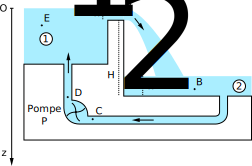
\includegraphics[scale=0.5]{meca_flu_bassin.pdf}
\end{center}

Une pompe $P$, située dans une canalisation de rayon $a\ll L$, refoule ensuite l'eau du bassin 2 dans le bassin 1 pour que l'eau reste en circuit fermé. La pompe de puissance $\dot{w}$ génère une surpression $\Delta P=P_D-P_C$ entre son entrée et sa sortie, et on supposera sa hauteur négligeable ($z_C\simeq z_D$). On prendra l'axe $z$ comme indiqué sur le schéma, avec $z$ croissant avec la profondeur et on notera $\rho$ la masse volumique de l'eau et $P_0$ la pression atmosphérique.

\begin{enumerate}

	\item L'écoulement est supposé parfait entre les lignes de courant $BC$, $DE$ et $EA$. Peut-on faire cette hypothèse sur les trajets $AB$ et $CD$ ? Conclure sur quels trajets il est possible d'appliquer le théorème de Bernoulli.

	%\item Déterminer les pressions $P_1(z)$ et $P_2(z)$ dans les bassins 1 et 2. On supposera que le champ de vitesse est négligeable dans les bassins, ceux-ci étant larges.
	
	%\item En déduire la vitesse de l'eau $v(z)$ au niveau du débordement (à la verticale du point $A$), puis le débit $D$ en fonction de $h_1$. 
	
	\item Les bassins étant larges, que peut-on dire sur la vitesse de l'eau au point $E$, loin du débordement ?
	
	\item En appliquant le théorème de Bernoulli entre les points $A$ et $E$ (supposés à la même altitude $z$), déterminer la vitesse de l'eau $v(z)$ au point $A$, au niveau du débordement, puis le débit de l'écoulement du bassin 1 vers le bassin 2.
	
	\item En appliquant judicieusement le théorème de Bernoulli sur différents trajets entre la surface du bassin 2 à celle du bassin A, expliciter une relation entre $\Delta P$ et les hauteurs $h_1$, $h_2$ et $H$.  Quelle surpression $\Delta P_{min}$ minimale doit fournir la pompe pour monter le niveau de l'eau du bassin 1 jusqu'à $z=h_1$ ?
	
	\item A l'aide d'un bilan d'énergie mécanique, montrer que la puissance fournie par la pompe s'écrit $\dot{w}=\Delta P\times D$. 
	
	\item Pourquoi la somme $h_1+h_2$ est une constante (de $h_1$ et $h_2$) ? En déduire la puissance $\dot{w}$ que doit fournir la pompe pour que l'eau atteigne une hauteur $h_1$ au-dessus du mur.

\end{enumerate}

\newpage

\begin{correction}

\begin{enumerate}

	\item Sur le trajet $AB$, l'écoulement est nécessairement turbulent pour que l'énergie cinétique de la chute soit dissipée (la vitesse en entrée de la canalisation $v_B=D/\pi a^2$ est indépendante de la vitesse de chute $\simeq\sqrt{2gH}$ puisque $H$ et la section $a$ peuvent être choisis indépendamment). 
	
	Sur le trajet $CD$, la pompe est là et génère aussi des turbulences ainsi que de l'énergie mécanique : Bernoulli n'est pas applicable.

	\item On applique la loi de la statique des fluide $P_1(z)$ et $P_2(z)$ dans les bassins 1 et 2 :
	\begin{align*}
		P_1(z) &= P_0+\rho g z, \quad z\in \mathrm{bassin 1} \\
		P_2(z) &= P_0+\rho g (z - (H + h_1)), \quad z\in [H + h_1 - h_2, H + h_1], \mathrm{bassin 2}
	\end{align*}
	
	\item On applique Bernoulli entre le point $A$, d'altitude $z$ au niveau du débordement, et le point $E$, situé à la même profondeur $z$, mais en plein dans le bassin. La pression en $A$ est celle de l'atmosphère, puisqu'il n'y a rien pour retenir l'eau (pas de paroi). La vitesse en $E$ est nulle, car on considère que la vitesse est négligeable dans les bassins. Enfin, $P_{E}=P_1(z)$.
	\begin{align*}
		\frac{\rho}{2}v_A^2+P_0=P_{1}(z)
	\end{align*}
	Donc, on retrouve le grand classique :
	\begin{align*}
		v(z) = \sqrt{2gz}
	\end{align*}	
	Le débit est alors :
	\begin{align*}
		D =& L\int_0^z\sqrt{2gz}dz \\
		=&\frac{2\sqrt{2g}}{3}Lh_1^{3/2}
	\end{align*}		
	
	\item La vitesse dans la canalisation est notée $v_c=D/\pi a^2$ par conservation du débit. \textbf{Attention : l'axe des $z$ est orienté vers le bas : il y a un signe - devant les termes en $\rho gz$}. En appliquant une première fois Bernoulli entre la surface du bassin 2 et le point $B$ :
	\begin{align*}
		 P_B-\rho g h_2 +\frac{\rho}{2}v^2 = P_0 
	\end{align*}
	Puis entre les trajets $BC$ et $CD$ on a les relations :
		\begin{align*}
		& P_B+\frac{\rho}{2}v^2-\rho g z_B = P_C+\frac{\rho}{2}v^2-\rho g z_C \\
		& P_D= P_C+\Delta P 
	\end{align*}
	Enfin, on applique Bernoulli entre $D$ et le point $E$ :
		\begin{align*}
		& P_D+\frac{\rho}{2}v^2-\rho g z_C= P_E-\rho g z_E = P_0
	\end{align*}	
	car $P_E=P_0-\rho g z_E$. On en déduit donc que (avec $z_B=H+h_1$) :
	\begin{align*}
		\Delta P = \rho g(H+h_1-h_2)
	\end{align*}
	On retrouve bien le cas statique : la vitesse n'intervient pas dans notre circuit. C'est normal : l'énergie cinétique acquise en entrant dans $B$ retourne sous forme de pression en sortant en arrivant dans le bassin 1.
	
	Dans le cas $h_1=0$, l'eau se situe à ras bord mais ne coule pas encore. On a donc $\Delta P_{min}=\rho g(H-h_2)$.
	
	\item On considère un volume de contrôle ouvert $V^\ast$ entre les points $C$ et $D$, ainsi qu'une masse $dm$ entrant en $C$ à l'instant $t$ et ressortant en $D$ à l'instant $t+dt$. L'énergie mécanique du système ${V_C; dm}$, qui est un système fermé s'écrit :
	\begin{align*}
		E(t)&=E_{V^\ast}-\rho g z_C + \frac{1}{2}dm v^2 \\
		E(t+dt)&=E_{V^\ast}-\rho g z_D + \frac{1}{2}dm v^2 \\
	\end{align*}
	Donc, ayant $z_C\simeq z_B$, on a $E(t+dt)-E(t)=0$. D'autre part, la variation d'énergie cinétique correspond au travail des forces de pression et de la pompe durant $dt$ :
	\begin{align*}
	E(t+dt)-E(t)=0=\dot{w}dt+P_C \pi a^2 v dt -P_D\pi a^2 v dt
	\end{align*}
	On trouve donc la relation voulue (comme $D=\pi a^2 v$) :
	\begin{align*}
		\dot{w} = D\Delta P 
	\end{align*}
	
	\item La quantité $L^2\times(h_1+h_2)=V$ représente le volume total du bassin, qui est constant, comme l'eau s'écoule en cycle fermé. Avec les relations précédentes :
	\begin{align*}
		\dot{w}&=\rho g(H+h_1-h_2)\frac{2\sqrt{2g}}{3}Lh_1^{3/2}\\
		&=\rho g(H'+2h_1)\frac{2\sqrt{2g}}{3}Lh_1^{3/2}
	\end{align*}
	avec $H'=H-V/L^2$. Seule solution : résolution graphique ou numérique.

\end{enumerate}

\end{correction}

\newpage

\section{Vidange d'un réservoir d'huile}

On considère un réservoir d'huile muni d'une ouverture de section circulaire $s=\pi r_0^2$ sur sa face inférieure, par laquelle s'écoule l'huile (supposée incompressible) sous l'action de la gravité. On définit l'axe vertical $Oz$ dirigé vers le bas, en prenant l'origine $O$ au niveau de l'ouverture. Une fois sorti du réservoir, on suppose qu'à la côte $z>0$, le filet d'huile a une section $\pi r(z)^2$ et que sa vitesse est uniforme et s'écrit ainsi $\vec{v}=v(z)\vec{e}_z$. D'autre part, le réservoir est un cylindre de rayon $R$ et de hauteur $H$.

\begin{center}
	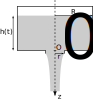
\includegraphics[scale=0.6]{meca_flu_huile.pdf}
\end{center}

\begin{enumerate}

\item On suppose dans un premier temps que la vitesse de l'huile à la sortie du réservoir est constante et égale à $v_0$.

\begin{enumerate}

	\item Déterminer la vitesse $v(z)$ de l'huile à la côte $z$.
	
	\item En déduire le rayon $r(z)$ du filet d'huile à la côte $z$. Simplifier la formule en considérant $v_0$ faible (devant quoi ?) pour obtenir $r(z)\propto 1/\sqrt[4]{z}$.
	
	\item Que représente le terme $\vec{v}\cdot\vv{\mathrm{grad}}(\vec{v})$ ? Le calculer et commenter. 
	
	\item Pourquoi l'expression de la vitesse est-elle incomplète ? A l'aide de la conservation locale du débit, montrer qu'elle doit s'écrire sous la forme $\vec{v}=v_r\vec{e}_r + v_z\vec{e}_z$ et déterminer la vitesse radiale $v(r,z)\vec{e}_r$ du filet l'huile en chute.

\end{enumerate}

\item On suppose désormais que le réservoir se vidange et que la hauteur d'huile, initialement au niveau $H$ dans le réservoir, diminue donc progressivement. On note  $h(t)$ la hauteur d'huile à l'instant $t$. 

\begin{enumerate}

	\item On note $v_1$ la vitesse de l'huile à la surface en $z=-h(t)$. Quel est le lien entre $v_1$ et la variation du niveau $\dot{h}(t)$ ? En déduire une relation $\dot{h}(t)$ et la vitesse $v_0(t)$.

	\item Quelle est la vitesse $v_0(t)$ de l'huile au niveau de l'ouverture en fonction de la hauteur $h(t)$, de $g$ et du rapport $\sigma=r_0^2/R^2$ ?
	
	\item En déduire la hauteur $h(t)$ en fonction du temps $t$.
	
	\item En combien de temps se sera vidé le réservoir ?

\end{enumerate}

\end{enumerate}

Expression de la divergence en coordonnées cylindriques :
\begin{align*}
	\mathrm{div}(\vec{v})=\frac{1}{r}\frac{\partial(rv_r)}{\partial r}+\frac{1}{r}\frac{\partial(v_\theta)}{\partial \theta}+\frac{\partial v_z}{\partial z}
\end{align*}
\newpage

\begin{correction}

\begin{enumerate}

\item

\begin{enumerate}

	\item Avec la formule de Torricelli (ou Bernoulli), on trouve que $v(z)=\sqrt{v_0^2+2gz}$.
	
	\item Conservation du débit volumique, en notant $D=\pi r_0^2v_0$ : $D= v(z)\pi r^2(z)$, donc :
	\begin{align*}
		r(z)&=\sqrt{\frac{r_0^2v_0}{\sqrt{v_0^2+2gz}}}\\
		&\simeq\sqrt{\frac{r_0^2v_0}{\sqrt{2g}}}z^{-\frac{1}{4}}
	\end{align*}
	
	\item Le terme se résume ici à : $\vec{v}\cdot\mathbf{grad}(\vec{v})=v_z\frac{\partial v_z}{\partial z}=g$. Il représente l'accélération convective, c'est-à-dire à un changement du champ de vitesse dans l'espace, qui est non-nulle malgré le caractère permanent de l'écoulement. L'accélération $\dot{V}(t)$ de la particule de poussière correspond à l'altitude $z$ à ce terme d'accélération convective. Il s'agit tout simplement d'une chute libre.
	
	\item La conservation du débit implique $\mathbf{div}(\vec{v})=0$. Or ici, le terme $\frac{\partial v_z}{\partial z}$ n'est clairement pas nul, donc pour cette forme d'écoulement cette condition n'est pas vérifiée. En réalité, lorsque le filet d'huile s'écoule, il s'allonge selon $z$ (à cause de l'accélération de la pesanteur) et doit donc, par conservation du volume, se contracter selon $r$ (c'est ce que l'on trouve avec un rayon qui décroit lors de la chute). Il y a donc nécessairement une vitesse du fluide selon $-\vec{e}_r$ pour qu'il s'amincisse : $\vec{v}=v_r\vec{e}_r + v_z\vec{e}_z$.
	
	En utilisant l'expression de la divergence, on a:
	\begin{align*}
		\frac{1}{r}\frac{\partial(rv_r)}{\partial r}=-\frac{g}{\sqrt{v_0^2+2gz}}
	\end{align*}
	Ainsi, on peut proposer :
	\begin{align*}
		v_r(r,z)=-\frac{1}{2}\frac{gr}{\sqrt{v_0^2+2gz}}
	\end{align*}
	Cette expression est cohérente : la vitesse est bien dirigée vers l'axe $Oz$, et décroit en fonction de $z$, comme $v_z$. On peut vérifier plus en détail : pour une particule de fluide située en $z$ sur le bord du filet d'huile, en $r(z)$, parcourt pendant $dt$ une distance $\vec{dl}=dr\vec{e}_r+dz\vec{e}_z$, avec $dr=v_r\cdot dt$ et $dz=v_z\cdot dt$. On doit donc avoir : $v_r/v_z=dr/dz$.
Commençons par calculer $dr/dz$ :
	\begin{align*}
		\frac{dr}{dz}&=\frac{d}{dz}\left(\sqrt{\frac{r_0^2v_0}{\sqrt{v_0^2+2gz}}} \right) \\
		&=-\sqrt{r_0^2v_0}\frac{g}{2}(v_0^2+2gz)^{-5/4} \\
		&=-\frac{g}{2}\sqrt{\frac{r_0^2v_0}{\sqrt{v_0^2+2gz}}}\frac{1}{v_0^2+2gz}\\
		&=-\frac{g}{2}\frac{r}{v_0^2+2gz}
	\end{align*}
	
	Donc :
	\begin{align*}
		v_r&=v_z\frac{dr}{dz} \\
		&=-\frac{1}{2}\frac{gr}{\sqrt{v_0^2+2gz}}
	\end{align*}
	

\end{enumerate}

\item

\begin{enumerate}

	\item On a tout simplement $v_1=-\dot{h}$. Avec la conservation du débit, on a $v_1\pi R^2=v_0\pi r_0^2$. Ainsi :
	\begin{align*}
		\dot{h}=-\sigma^2 v_0
	\end{align*}

	\item On utilise Bernoulli entre la surface de l'huile ($z=z_1$, où la pression est $P_0$) dans le réservoir et au niveau de l'orifice ($z=0$, où la pression est aussi $P_0$, étant à l'air libre) :
	\begin{align*}
		P_0-\rho gz_1+\rho\frac{1}{2}v_1^2=P_0-\rho gz_2+\rho\frac{1}{2}v_0^2
	\end{align*}
	Donc :
	\begin{align*}
		v_0(t)^2=\frac{2g}{1-\sigma^2}h(t)
	\end{align*}
	
	\item Comme $\dot{h}=-\sigma^2 v_0$, on a l'équation différentielle suivante :
	\begin{align*}
	 	-\dot{h}=\sqrt{\frac{2g\sigma^2}{1-\sigma^2}}\sqrt{h(t)} 
	\end{align*}
	La solution est :
	\begin{align*}
		h(t)=\left( \frac{1}{2}\sqrt{\frac{2g\sigma^2}{1-\sigma^2}}t-\sqrt{H}\right)^2
	\end{align*}
	
	\item Le réservoir ce sera vidé lorsque $h(t)=0$, cad pour $t=T$ :
	\begin{align*}
		T=\sqrt{\frac{2(1-\sigma^2)H}{2g\sigma^2}}
	\end{align*}

\end{enumerate}

\end{enumerate}

\end{correction}

\newpage

\section{Écoulement d'un fluide en pente}

Un fluide de forte viscosité ($\eta$, masse volumique $\rho$), d'épaisseur $h$, est soumis à la gravité (notée $\vec{g}$) s'écoule lentement sur un plan infini incliné d'un angle $\alpha$ par rapport à la verticale. On se place en régime permanent, on suppose que la vitesse selon $\vec{e}_y$ est nulle et que le fluide est incompressible. On cherche à décrire l'écoulement de ce fluide.

\begin{center}
	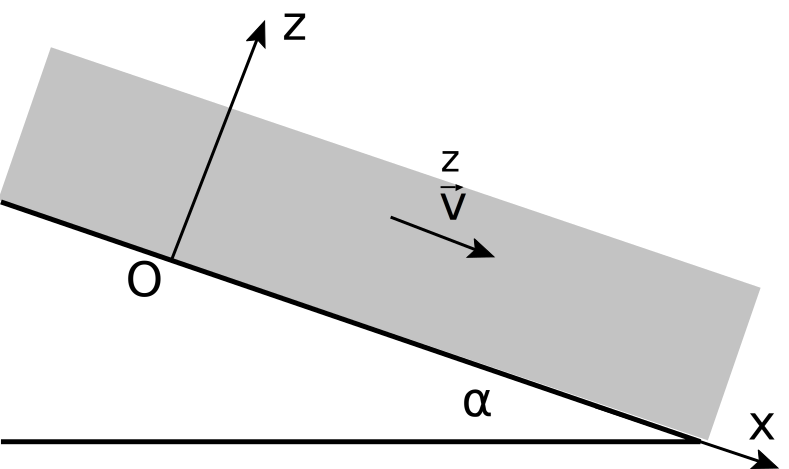
\includegraphics[scale=0.4]{meca_flu_ecoulement.pdf}
\end{center}

\begin{enumerate}

	\item Montrer que $\vec{v}(x,y,z)=v(z)\vec{e_x}$. 
	
	\item Écrire le bilan des forces volumiques s'exerçant sur un volume de fluide situé au point $M=(x,y,z)$.
	
	\item En déduire le profil de vitesse dans le fluide.
	
	\item En déduire le débit linéique (le débit par unité de longueur selon l'axe $y$).
	
	\item On souhaite avoir un ordre de grandeur de la viscosité d'un glacier. Pour cela, dispose d'image satellite du glacier du Tacul, situé sur la face nord du Mont Blanc. Chaque "rayure" correspond à une année. Estimer sa viscosité. 
	
\begin{center}
	\includegraphics[scale=1]{meca_flu_glacier.png}
\end{center}


	\item En reprenant la première figure, on place désormais une plaque au dessus du liquide, au niveau de $z=h$. Que deviennent les conditions aux limites ? Trouver le nouveau profil de vitesse. Comment s'appelle se type d'écoulement ?

\end{enumerate}

\newpage

\begin{correction}

\begin{enumerate}

	\item Comme l'écoulement est lent, et invariant selon $x$ et $y$ : l'écoulement ne dépend que de $z$. De plus, comme il est incompressible, $div(\vec{v})=0$, donc $v_z=cste=0$, car la vitesse doit être nécessairement nulle en $z=0$. L'écoulement est donc laminaire et est dirigé selon $\vec{e_x}$ (c'est une hypothèse, on suppose qu'il est dans le sens de la descente) : $\vec{v}(x,y,z)=v(z)\vec{e_x}$.
	
	\textit{NB : }avec un tel profil de vitesse, $(\vec{v}\cdot\vec{grad})\vec{v}$ est identiquement nul, mais on peut directement le négliger ce terme avec l'hypothèse de l'énoncé (écoulement lent et très visqueux).
	
	\item Les forces s'exerçant sur le fluide sont celles de gravité, de pression et de viscosité. Le bilan des forces s'écrit : 

\begin{align*}
	0=\eta \Delta \vec{v}+\rho\vec{g}-\vec{grad}(P)
\end{align*}

	En projetant sur les axes $x$ et $z$, on obtient :
	
\noindent\fbox{\parbox{\linewidth\fboxrule-2\fboxsep}{
\begin{equation}
\left\lbrace
\begin{array}{ccc}
\vec{e_x}  & : & \eta\frac{\partial^2 v}{\partial z^2}+\rho g \sin\alpha - \frac{\partial P}{\partial x}=0\\
\vec{e_z}  & : &-\rho g \cos\alpha - \frac{\partial P}{\partial z}=0\\
\end{array}\right.
\end{equation}	
}}

	\item En intégrant selon $\vec{e_z}$ et avec la condition au limite $P(x,z=h)=P_0$, on obtient :
\begin{align*}
	P(x,z)=P_0+\rho g\cos\alpha (h-z)
\end{align*}
En intégrant selon $\vec{e_x}$, avec la condition aux limites $\frac{\partial v}{\partial z}_{z=h}=0$ (il n'y a pas de forces de cisaillement à l'interface air/fluide) devient alors : 
\begin{align*}
	\frac{\partial v}{\partial z}=\frac{\rho g}{\eta}\sin\alpha(h-z)
\end{align*}
En intégrant une nouvelle fois, avec la condition aux limites $v(z=0)=0$ (continuité  de la vitesse avec le support) :

\noindent\fbox{\parbox{\linewidth\fboxrule-2\fboxsep}{
\begin{align*}
	v(z)=\frac{\rho g}{\eta}\sin\alpha z\left( h-\frac{z}{2}\right) 
\end{align*}
}}

Le profil de vitesse est parabolique.

\item Le débit s'écrit, en prenant comme section un carré de largeur $L\gg h$ pour que les hypothèses de l'énoncé soient valables : 
\begin{align*}
	D=\int_{y=0}^{L}dy\int_{z=0}^h dz\cdot v(z)
\end{align*}
En intégrant, on obtient :

\noindent\fbox{\parbox{\linewidth\fboxrule\fboxsep}{
\begin{align*}
	D=\frac{\rho g}{3\eta}\sin\alpha L h^3
\end{align*}
}}

\item La glace a une densité de 900kg.m$^3$. La vitesse proposée est la vitesse maximale de la glace, car c'est celle en surface. On a donc $\eta\simeq7.1\cdot10^{12}$Pa.s.

On obtient donc, sur une année : $V=D\Delta t\simeq4,73\cdot10^6$m$^3$, soit 4250 tonnes chaque année. 

Il faut garder à l'esprit que ce sont des ordre de grandeurs, car nous n'avons pas pris en compte les conditions aux limites sur les bords (en $y$) du canal d'écoulement du glacier, et que la vitesse est elle aussi un ordre de grandeur. 

\item[$\blacktriangleright$] Les conditions aux limites deviennent alors $v(z=0)=v(z=h)=0$, mais on a plus la condition sur la dérivée première de la vitesse. 
La vitesse s'écrit : $v(z)=-\frac{\rho g}{2\eta}\sin\alpha z^2 +a +b$
Avec les conditions aux limites, on trouve $b=0$ et $a=\frac{\rho g}{2\eta}\sin\alpha h$.

\noindent\fbox{\parbox{\linewidth\fboxrule-2\fboxsep}{
\begin{align*}
	v(z)=\frac{\rho g}{2\eta}\sin\alpha z\left( h-z\right) 
\end{align*}
}}

C'est un écoulement de Poiseuille. 

\end{enumerate}

\end{correction}

\newpage

\section{Boîte automatique}

On modélise un convertisseur de couple d'une boite automatique, dispositif permettant de se passer d'un embrayage, comme un système de deux cylindres de même axe $\vec{e}_z$, et de rayons respectifs $R_1$ et $R_2$, de longueur $L$, entre lesquels se trouve un fluide de viscosité $\eta$ élevée (\textit{schéma de gauche}). Le moteur (resp. l'arbre de transmission) est solidaire du cylindre $1$ (resp. 2) et tourne à la vitesse $\Omega_1$ (resp. $\Omega_2$). Lorsque le moteur fournit un couple $\Gamma_1$ au cylindre 1, il entraîne le fluide situé entre $R_1$ et $R_2$, qui entraîne à son tour le cylindre 2, relié à la boite de vitesse. Pour étudier son fonctionnement, on se placera en coordonnées cylindriques. 

\begin{center}
	\includegraphics[scale=0.8]{meca_flu_boite_auto.pdf}
\end{center}

On rappelle que la force surfacique de viscosité, entre deux couches élémentaires 1 et 2 adjacentes de fluide, s'écrit : $\vec{\sigma}_{1\rightarrow2}=\frac{d\vec{F}_{1\rightarrow2}}{dS}$, où $d\vec{F_{1\rightarrow2}}$ est la force exercée de la couche 1 sur la couche 2,  $dS$ étant la surface élémentaire de contact (\textit{schéma de droite}). On admet que son expression en coordonnées cylindriques de sa composante selon $\vec{e_\theta}$ s'écrit : 
\begin{align*}
	\sigma_\theta(r,\theta,z)=\eta\left(\frac{1}{r}\frac{\partial v_r}{\partial \theta}+ \frac{\partial v_\theta}{\partial r} - \frac{v_\theta}{r} \right)
\end{align*}

On admet que les autres composantes de $\vec{\sigma}$ sont nulles ($\sigma_r=\sigma_z=0$). On suppose par ailleurs que l'écoulement est incompressible et permanent, que la vitesse ne dépend que de $r$, et enfin que $v_z=0$.

\begin{enumerate}

\item

\begin{enumerate}
		
	\item Quel est le nombre de Reynolds de cet écoulement ? En déduire le type d'écoulement. 
	
	\item Montrer que le champ de vitesse est strictement orthoradial : $\vec{v}=v_\theta (r)\vec{e_\theta}$.
	
	\item En faisant un bilan des moments sur un élément de fluide selon $\vec{e_z}$ et en négligeant les forces de pression, montrer que la vitesse vérifie la relation suivante : 
	\begin{align*}
		\frac{\partial}{\partial r}\left(r^3 \frac{\partial}{\partial r}\frac{v_\theta}{r} \right) =0
	\end{align*}
	
	\item A l'aide des conditions aux limites, en déduire l'expression du champ de vitesse $\vec{v}$.
	
	\item Calculer le couple $\Gamma_{1\rightarrow2}$ qu'exercent les forces visqueuses sur le cylindre 2. Comparer avec $\Gamma_{2\rightarrow1}$.
 \end{enumerate}

\item On suppose que le moteur peut asservir son régime moteur de sorte à garder $\Omega_1$ fixé, quelque soit le couple $\Gamma_{1\rightarrow2}$ qu'il délivre.

\begin{enumerate}
	
	\item Le véhicule roule à vitesse constante dans une montée, équivalent à un couple résistif $-\Gamma_r$ sur l'arbre de transmission. Déterminer $\Omega_2$ puis le rendement du convertisseur de couple. Quels sont les intérêts et les inconvénients d'un convertisseur de couple par rapport à un embrayage classique ?
	
	\item  Désormais, le véhicule est initialement à l'arrêt, et démarre à pleine puissance sur une route plate à $t=0$. L'inertie du véhicule est vue au niveau du cylindre 2 comme un moment d'inertie $J$. Déterminer l'évolution $\Omega_2(t)$. 
		
\end{enumerate}

\end{enumerate}


\textit{Données :} $R_1=295$mm, $R_2=300$mm, $L=500$mm, $\rho=860$kg.m$^{-3}$ et $\eta=120$ SI. 
\begin{align*}
	\mathrm{div}(\vec{A}) =
\frac{1}{r}\frac{\partial (r A_r)}{\partial r} + \frac{1}{r}\frac{\partial A_\theta}{\partial \theta} + \frac{\partial A_z}{\partial z}
\end{align*}	


\newpage

\begin{correction}

\begin{enumerate}

\item

\begin{enumerate}
		
	\item Question piège : on a pas la vitesse de rotation. Pour un moteur de voiture, on a typiquement $\Omega=1000$tr/min$\simeq105$rad/s, soit une vitesse typique $U=R_2\Omega\simeq31$m/s. On trouve $Re=\rho UL/\eta\simeq 67$, soit un écoulement laminaire.
	
	\item Comme l'écoulement est incompressible, on a $\mathbf{div}(\vec{v})=0$. Avec les hypothèses de l'énoncé, on trouve donc que $v_r=\frac{cste}{r}$. Comme $v_r(R_1)=0$ par conservation du débit, $\forall r, v_r=0$.
	
	\item Le plus simple est de faire un bilan des moments selon $\vec{e_z}$ à un élément de fluide (en coordonnées cylindriques) qui est un anneau (ou tore) compris entre $r$ et $r+dr$, d'épaisseur $dz$. Les forces visqueuses s'appliquent orthoradialement alors sur les surfaces internes et externe. 

Comme on est en régime stationnaire, le moment total exercé doit être nul de sorte que : 
\begin{align*}
	2\pi r dz \sigma_\theta(r)\times r - 2\pi (r+dr) dz \sigma_\theta(r+dr)\times (r+dr) = 0
\end{align*}
cad : $r^2 \sigma_\theta(r) - (r+dr)^2 \sigma_\theta(r+dr) = 0$. On en déduit que $\frac{\partial}{\partial r}r^2\sigma_\theta=0$.

D'autre part, $\sigma_\theta=\eta\left(\frac{\partial v_\theta}{\partial r}-\frac{v_\theta}{r}\right) =\eta r \frac{\partial}{\partial r}\frac{v_\theta}{r} $. On trouve le résultant voulu :

\noindent\fbox{\parbox{\linewidth\fboxrule-2\fboxsep}{	
	\begin{align*}
		\frac{\partial}{\partial r}\left(r^3 \frac{\partial}{\partial r}\frac{v_\theta}{r} \right) =0
	\end{align*}}}
	
	\item On intègre la relation précédente et on trouve :
	\begin{align*}
		v_\theta = \frac{A}{r} + Br
	\end{align*}
	Les conditions aux limites sont : $v_\theta(r=R_{1,2})=R_{1,2}\Omega_{1,2}$. On obtient alors : 
	
	\noindent\fbox{\parbox{\linewidth\fboxrule-2\fboxsep}{	
	\begin{align*}
		v_\theta  = -\frac{(\Omega_2-\Omega_1)R_2^2R_1^2}{R_2^2-R_1^2}\frac{1}{r}+\frac{\Omega_2R_2^2-\Omega_1R_1^2}{R_2^2-R_1^2}r
	\end{align*}}}
	
	\item Le couple s'exerçant sur une surface élémentaire $dS=R_2\cdot d\theta\cdot  dz$ du cylindre 2 correspond au moment des forces de cisaillement en $R_2$ : $d\Gamma_{1\rightarrow2} = \sigma_\theta(R_2)\cdot dS\cdot R_2$.
	
	Comme $\sigma_\theta(r)=\eta r \frac{\partial}{\partial r}\frac{v_\theta}{r}=-2\eta\frac{A}{r^2}$, on a :
	
	\begin{align*}
		\Gamma_{1\rightarrow2}	 = -4\pi\eta L\frac{(\Omega_2-\Omega_1)R_2^2R_1^2}{R_2^2-R_1^2}
	\end{align*}
	
	On trouve bien que le couple reçu par 2 $\Gamma_{1\rightarrow2}$ est négatif lorsque $\Omega_2>\Omega_1$, et inversement.
	
	Pour le cas du cylindre 1, le calcul donne la même chose, avec un signe négatif (car les forces de viscosité s'exercent sur un cylindre plus petit) :
	
		\begin{align*}
		\Gamma_{2\rightarrow1}	 =4\pi\eta L\frac{(\Omega_2-\Omega_1)R_2^2R_1^2}{R_2^2-R_1^2}
	\end{align*}
	
	On trouve bien que $\Gamma_{1\rightarrow2} + \Gamma_{2\rightarrow1}	=0$. Le couple exercée par le cylindre 1 est bien reçu par le cylindre 2, et inversement.
	
	\end{enumerate}
	
	\item
	
	\begin{enumerate}
	
	\item En supposant que la vitesse de rotation du moteur est fixée à $\Omega_1$, déterminer $\Omega_2$. Calculer alors la puissance dissipée dans le fluide visqueux et la comparer avec la puissance mécanique $P_1$ fournie par le moteur et $P_2$, celle récupérée par l'arbre de transmission.
	
	Le couple résistif s'exerce sur l'arbre de transmission, cad sur le cylindre 2, donc le couple résistif s'exerce aussi sur 1 : $\Gamma_{2\rightarrow1} = -\Gamma_r$. On trouve donc :
	
	\begin{align*}
		-\Gamma_{r}	 =4\pi\eta L\frac{(\Omega_2-\Omega_1)R_2^2R_1^2}{R_2^2-R_1^2}
	\end{align*}
	cad :
	\begin{align*}
		\Omega_2 =\Omega_1 - \frac{\Gamma_{r}}{4\pi\eta L}\frac{R_2^2-R_1^2}{R_2^2R_1^2}<\Omega_1
	\end{align*}
	On trouve que l'arbre extérieur tourne moins vite que l'arbre intérieur : le couple résistif fait "glisser" le convertisseur de couple. Si le couple résistif est trop important, on peut même arrêter l'arbre de transmission : le véhicule s'arrête ! 
	
	Par ailleurs, toute la puissance n'est pas transmise à l'arbre 2. La puissance fournie par le moteur est $P_1 = \Omega_1\Gamma_r$ et la puissance reçue par l'arbre est $P_2 = \Omega_2\Gamma_r<P_1$. Le rendement du convertisseur est alors :
	\begin{align*}
		r = \frac{P_2}{P_1} = \frac{\Omega_2}{\Omega_1}=1-\frac{\Gamma_{r}}{4\pi\eta L\Omega_1}\frac{R_2^2-R_1^2}{R_2^2R_1^2}
	\end{align*}
	
	Le rendement est systématiquement inférieur à 1, sauf lorsqu'il n'y a pas de couple résistif.
	
	On a bien vu que, par essence, ce convertisseur de couple perd de la puissance par dissipation dès qu'il doit exercer un couple ou transmettre de la puissance. Néanmoins, l'avantage est que le moteur peut rester à régime fixe (notamment sur les meilleures plages de rendement) et il n'y a pas de discontinuité dans la transmission du couple, contrairement à un embrayage (lorsqu'on change de vitesse : les disques se décollent et frottent par ailleurs aussi). Un embrayage fonctionnant sur le même rapport n'a aucune perte.
		
\end{enumerate}

\end{enumerate}

\end{correction}

\newpage

\section{Augmenter la vitesse du jet d'eau à la sortie d'un tuyau (\textit{PSI})}

Dans un jardin, un tuyau d'arrosage de longueur $L$ et de diamètre constant $d_B=2$ cm est branché sur une arrivée d'eau en $A$, connectée à un réservoir de taille très grande où la pression en $O$ (loin de $A$) est $P_1=3$ bar. A l'autre extrémité du tuyau, on dispose d'un rétrécissement (entre les points $B$ et $C$, de longueur négligeable), faisant passer le diamètre de $d_B$ à $d_C$. On note $\sigma=d_C/d_B$. La pression en sortie de tuyau (au point $C$) est la pression atmosphérique $P_0=1$ bar.

\begin{center}
	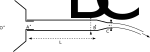
\includegraphics[scale=1.0]{meca_flu_tuyau.pdf}
\end{center}

\begin{enumerate}

	\item Si l'écoulement était parfait, quelle serait la vitesse $U_T$ (dite vitesse de Torricelli) du jet d'eau à la sortie en $C$ ? Est-ce que le rétrécissement joue un rôle ?
	
	\item Quel est le nombre de Reynolds associé à cet écoulement ? On rappelle que pour l'eau $\eta = 1,0\times 10^{-3}$ SI et $\rho=1,0\times 10^3$. En déduire le type d'écoulement auquel on a affaire. Est-il parfait ? Quel phénomène doit-on prendre en compte ?
	
	\item Rappeler l'expression des pertes de charges $\Delta_A^B P$ dans le tuyau, entre $A$ et $B$, en fonction de la vitesse débitante dans le tuyau $U_B$, $\rho$, $L$, $d_B$, et $\xi$ le coefficient de perte de charge donné par le diagramme de Moody. En déduire, dans le cas $\sigma=1$, l'expression de la vitesse $U_C$ à la sortie du tuyau. Application numérique pour $L=4$m, et une rugosité relative du tuyau de $\varepsilon=0,01$.
	
	\item Le rétrécissement provoque une perte de charge que l'on peut écrire sous la forme :
	\begin{align*}
		\Delta_B^CP=-\frac{1}{2}\rho\left(1-\sigma^2\right) \chi U_C^2
	\end{align*}
avec $\chi=0,3$. Montrer que la vitesse de sortie s'écrit sous la forme :
\begin{align*}
	U_C=\frac{U_T}{\sqrt{\alpha+\beta\sigma^2+\gamma\sigma^4}} 
\end{align*}
et déterminer les constantes $\alpha$, $\beta$ et $\gamma$.

\item A quelle condition sur la longueur $L$ du tuyau la vitesse du jet d'eau augmente d'elle lorsqu'on réduit le diamètre de sortie $d_C$ ? Le débit augmente t-il ?

\end{enumerate}

\newpage

\begin{correction}

\begin{enumerate}

\item On applique Bernoulli entre les points $O$ et $C$, on trouve que la vitesse de sortie est $U_T=\sqrt{2\Delta P/\rho}$, où $\Delta P=P_1-P_0=2$ bar. On trouve $U_T=20$m/s. Elle ne dépend pas de la largeur de la sortie, le rétrécissement en joue aucun rôle.

\item On trouve $Re=4\times10^5$. On est donc dans un écoulement turbulent, il n'est pas parfait et on doit prendre en compte les pertes de charges.

\item Les pertes de charges régulières s'écrivent sous la forme :
\begin{align*}
	\Delta P_r = \frac{1}{2}\frac{L}{d_B}\rho\xi U_B^2
\end{align*}
Avec le diagramme de Moody, on trouve $\xi\simeq 0,04$.
On a donc, en tenant compte des pertes : 
\begin{align*}
	P_O+\frac{1}{2}\rho v_O^2=P_A+\frac{1}{2}\rho v_B^2 + \Delta P_r 
\end{align*}
On obtient donc une équation sur $U_B=U_C$ :
\begin{align*}
	\Delta P -\frac{1}{2}\frac{L}{d_B}\rho\xi U_B^2=\frac{1}{2}\rho U_C^2
\end{align*}
On voit bien que la perte de charge diminue la vitesse par rapport à l'écoulement parfait. On trouve ainsi :
\begin{align*}
	U_B&=\frac{U_T}{\sqrt{1+\frac{\xi L}{d_B}}} \\
	&=\frac{U_T}{3}
\end{align*}
Cad $U_T=6,7$m/s.

\item On réapplique Bernoulli entre $O$ et $C$ avec cette perte de charge :
\begin{align*}
P_O+\frac{1}{2}\rho U_O^2=P_C +\frac{1}{2}\rho U_C^2 + \Delta_O^B  P+\Delta_B^C P \\
\end{align*}
Ce qui devient :
\begin{align*}
	P_O-P_C = \Delta P &=\frac{1}{2}\frac{L}{d_B}\rho\xi U_B^2+\frac{1}{2}\rho\left(1-\sigma^2\right) \chi U_C^2 +\frac{1}{2}\rho U_C^2\\
	&=\frac{1}{2}\rho U_C^2\left(1+\frac{L}{d_B}\xi\sigma^4 +\chi\left(1-\sigma^2\right) \right) 
\end{align*}

\textbf{Attention ! } : la chute de pression n'est pas uniquement due aux pertes de charges causée par les turbulences, comme une loi des séries des résistances hydrauliques. L'accélération du fluide entre $O$ et $A$, puis entre $B$ et $C$ génère aussi une baisse de la pression à cause de l'accélération du fluide (effet Venturi). 

On isole alors la vitesse en sortie de tuyau :
\begin{align*}
	U_C&=\frac{U_T}{\sqrt{1+\frac{L}{d_B}\xi\sigma^4 +\chi\left(1-\sigma^2 \right) }} \\
	&=\frac{U_T}{\sqrt{\alpha+\beta\sigma^2+\gamma\sigma^4}}
\end{align*}
avec $\alpha=1+\chi$, $\beta=-\chi$ et $\gamma=L\xi/d_B$.

\item On regarde les cas extrêmes $\sigma\rightarrow0$ et $\sigma\rightarrow1$. On trouve :
\begin{align*}
	U_C(\sigma\rightarrow1)=\frac{U_T}{\sqrt{\left(1+\frac{L}{d_B}\xi \right) }}
\end{align*}
On retombe bien sur le résultat de la question précédente : il n'y a que les pertes de charges régulières. 

\begin{align*}
	U_C(\sigma\rightarrow0)=\frac{U_T}{\sqrt{\left(1+\chi\right) }}
\end{align*}
Dans ce cas-là, il n'y a que la perte de charge singulière due au rétrécissement, car la vitesse $U_B$ dans le tuyau tend vers 0.

Pour que la vitesse du jet augmente lorsqu'on rétrécit la sortie, il faut que $U_C(\sigma\rightarrow0)>U_C(\sigma\rightarrow1)$, c'est-à-dire :
\begin{align*}
	L>\frac{\chi d_B}{\xi}
\end{align*}

{\centering \includegraphics[scale=0.7]{meca_flu_tuyau2.png} \par}

\end{enumerate}

\end{correction}

\newpage

\section{Écoulement de Poiseuille cylindrique}

Un capillaire sanguin est un vaisseau sanguin très fin, dans lequel circule du sang, supposé être un fluide incompressible de masse volumique $\rho=1,0\times10^3$kg.m$^{-3}$ et de viscosité $\eta=4\times10^{-2}$ Pa.s. Le capillaire peut être modélisé comme un tuyau cylindrique, de rayon $R=10$ microns et de longueur $L\gg R$ suivant l'axe $z$. La pression artérielle impose une différence de pression $\Delta P = P_e-P_s$ à ses extrémités, entre $z=0$ et $z=L$. On se place en coordonnées cylindriques dans tout l'exercice, en notant $O$ l'origine du repère. On néglige dans tout l'exercice le poids du fluide et on suppose l'écoulement stationnaire.

\begin{enumerate}

	\item Estimer le nombre de Reynolds pour cet écoulement, alors que l'ordre de grandeur de la vitesse est de 1mm/s. En déduire le type d'écoulement auquel on a affaire, et justifier que le champ de vitesse s'écrit sous la forme $\vec{v}=v_z(r)\vec{e}_z$.

	\item On considère un volume élémentaire $d\tau=rd\theta\times dr\times dz$ de fluide situé en $\vv{OM}=r\vec{e}_r+z\vec{e}_z$. Quelles forces s'appliquent sur ce volume ? Donner leur expression en coordonnées cylindriques. 
	
	\item En déduire que la vitesse vérifie la relation suivante : 
	\begin{align*}
		\eta\frac{\partial}{\partial r}\left( r\frac{\partial v_z(r)}{\partial r}\right) -\frac{r\Delta P}{L}=0
	\end{align*}

	\item En supposant qu'il n'y a pas de glissement en $r=R$, montrer que la vitesse s'écrit alors :
	\begin{align*}
		v_z(r)=v_0\left(1-\frac{r^2}{R^2} \right) 
	\end{align*}
	Expliciter $v_0$.
	
	\item En déduire le débit volumique $D_v$ de cet écoulement, ainsi que la vitesse débitante $U$ associée. 
	
	\item \textit{(PSI)} Montrer que le coefficient de perte de charge que l'on peut trouver dans le diagramme de Moody s'écrit $\xi=64/Re$ pour cet écoulement.
		
\end{enumerate}

\newpage

\begin{correction}

\begin{enumerate}

	\item Ici $Re=10^{-2}$, on a donc un écoulement laminaire (très visqueux). L'écoulement étant laminaire, la vitesse est nécessairement orientée selon l'axe du tuyau $\vec{e}_z$. D'autre part, le problème étant invariant par translation le long de l'axe $e_z$ et par rotation autour de $\vec{e}_\theta$, la vitesse ne dépend que de $r$.

	\item Les forces de pression et de viscosité s'appliquent le volume élémentaire $d\tau=rd\theta\times dr\times dz$. Respectivement, il y a la force de pression sur la face en $z$, la force de pression en $z+dz$, la force de viscosité en $r$ et celle en $r+dr$, soit :
	\begin{align*}
		P(z)\times rd\theta\times dr - P(z+dz)\times rd\theta\times dr - \eta\frac{\partial v_z}{\partial r}(r)\times rd\theta\times dz + \eta\frac{\partial v_z}{\partial r}(r+dr)\times (r+dr)d\theta\times dz=0
	\end{align*}
	
	\item L'équation précédente donne :
	\begin{align*}
		-rd\theta\times dr\times dz\frac{\partial P}{\partial z}+\eta\frac{\partial}{\partial r}\left( r\frac{\partial v_z(r)}{\partial r}\right) dr\times d\theta\times dz=0
	\end{align*}
	et donc, en intégrant sur $z$ de $0$ à $L$ :
	\begin{align*}
		\eta\frac{\partial}{\partial r}\left( r\frac{\partial v_z(r)}{\partial r}\right) -\frac{r\Delta P}{L}=0
	\end{align*}

	\item On intègre cette équation deux fois, on trouve facilement avec la condition limite que :
	\begin{align*}
		v_z(r)=v_0\left(1-\frac{r^2}{R^2} \right) 
	\end{align*}
	avec $v_0=R^2\Delta P/4\eta L$
	
	\item Le débit volumique s'écrit :
	\begin{align*}
		D_v&=\iint rd\theta drv_z(r) \\
		&=2\pi\times\int rdrv_0\left(1-\frac{r^2}{R^2} \right) \\
		&=\pi R^2\frac{v_0}{2} 
	\end{align*}
	
	La vitesse débitante (définie comme le rapport du débit sur la surface) est donc $U=v_0/2$.
	
	\item \textit{(PSI)} La perte de charge s'écrit $\Delta P=\frac{1}{2}\frac{L}{D}\rho\xi U^2$.
	On a donc :
	\begin{align*}
		\Delta P = \xi\frac{L}{4R}\rho U\frac{\Delta P R^2}{8L\eta}
	\end{align*}
	Donc :
	\begin{align*}
		\xi = \frac{64 \eta}{\rho U D}
	\end{align*}
		
\end{enumerate}

\end{correction}

\newpage

\begin{center}
	\includegraphics[scale=1.5]{meca_flu_moody.png}
\end{center}

\newpage

\section{Lancer de javelot \textit{(PSI)}}

Un athlète lance un javelot (masse $m=0,8$kg, diamètre $d=$4cm, longueur $l=$2m) avec une vitesse initiale $V_0=30$m.s$^{-
1}$ depuis la position $(x_0, z_0)=(0,0)$. Une fois en vol, à l'instant $t$, le javelot  se déplace a une vitesse $\vec{V}(t)$ et est repéré par sa position horizontale $x(t)$ et verticale $z(t)$, ainsi que par l'angle entre son axe et l'horizontale, $\alpha(t)$. On note par ailleurs $p(t)$ l'angle entre $\vec{V}(t)$ et l'horizontale, et $i(t)$ l'angle entre l'axe du javelot et $\vec{V}(t)$ (\textit{figure de gauche}).

\begin{figure}[h!]
   \begin{minipage}[c]{.46\linewidth}
      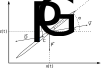
\includegraphics[scale=0.85]{meca_flu_javelot.pdf}
   \end{minipage} \hfill
   \begin{minipage}[c]{.46\linewidth}
      \includegraphics[scale=0.65]{meca_flu_coeff_aero.pdf}
   \end{minipage}
\end{figure}

On suppose que les forces aérodynamiques de portance et de trainée, notées respectivement $\vec{L}$ et $\vec{D}$, s'appliquent au centre de pression, au point $C_P$, à une distance $l$ du centre de gravité $C_G$, où s'applique le poids $\vec{P}$.

On note $\rho=1,17$kg.m$^{-3}$ la masse volumique de l'air, $\eta=1,85\times10^{-5}$ Pa.s sa viscosité, $g$ l'accélération de la pesanteur, $S$ la surface du javelot, $C_x(i)$ et $C_z(i)$ les coefficients de trainée et de portance, que l'on suppose dépendre de l'angle $i$.

\begin{enumerate}

	\item Quel est le nombre de Reynolds associé à cet écoulement ? En déduire le type d'écoulement. Rappeler alors l'expression de $L$ et $D$, normes des forces de portance et de trainée, en fonction de $\rho$, $S$, $C_x$, $C_z$ et de $V$, la norme de la vitesse.
	
	\item Une mesure expérimentale (\textit{figure de droite}) permet d'obtenir les courbes de $C_x$ et de $C_z$ en fonction de l'angle d'incidence $i$. Identifier à quelle courbe correspond $C_x$ et $C_z$. En utilisant les symétries du problème, déterminer l'allure des courbes pour des angles d'incidence négatifs.

	\item Dans quelle direction pointent respectivement $\vec{L}$ et $\vec{D}$ ? En déduire leur expression vectorielle sous la forme $\vec{L}=L_x\vec{e}_x+L_z\vec{e}_z$ et $\vec{D}=D_x\vec{e}_x+D_z\vec{e}_z$.
	
	\item A l'aide d'un PFD, montrer que l'équation du mouvement du javelot s'écrit :
	\begin{align*}
		m\ddot{x} &= -\frac{1}{2}\rho SC_z(i)\dot{z}\sqrt{\dot{x}^2+\dot{z}^2}-\frac{1}{2}\rho SC_x(i)\dot{x}\sqrt{\dot{x}^2+\dot{z}^2} \\
		m\ddot{z} &= -mg+\frac{1}{2}\rho SC_z(i)\dot{x}\sqrt{\dot{x}^2+\dot{z}^2}-\frac{1}{2}\rho SC_x(i)\dot{z}\sqrt{\dot{x}^2+\dot{z}^2}
	\end{align*}
	
	\item En notant $J$ le moment d'inertie du javelot autour de l'axe $y$, montrer à l'aide du théorème du moment cinétique que l'on a :
	\begin{align*}
		J\ddot{\alpha} &= -\frac{1}{2}\rho S(\dot{x}^2+\dot{z}^2)(C_z(i)\cos(i)+C_x(i)\sin(i))
	\end{align*}
	
	En déduire que l'on peut alors déterminer la trajectoire du javelot au cours du temps avec les 5 variables du problème ($x$, $z$, $\alpha$, $i$ et $p$) à l'aide d'une simulation numérique.
	

\end{enumerate}

\newpage

\begin{correction}

\begin{enumerate}

	\item On trouve $Re=\rho VL/\eta\simeq 76 000$, c'est un écoulement turbulent. Dans ces conditions, les forces de trainées et de portance s'écrivent respectivement :
	\begin{align*}
		D&=\frac{1}{2}\rho SC_x(i)V^2 \\
		L&=\frac{1}{2}\rho SC_z(i)V^2
	\end{align*}
	
	\item On remarque que le coefficient de portance $C_x$ démarre à 0 : c'est normal, car le javelot étant symétrique par rapport au vent à $i=0$, il ne doit pas y avoir de force de portance. A l'inverse, le coefficient de trainée commence à une valeur non-nulle, car la trainée est nécessairement non nulle quelque soit l'angle d'incidence. 
	D'autre part, la portance augmente avec l'incidence : le javelot se comporte comme une aile symétrique, en repoussant le flux d'air incident selon les $z$ négatifs. La trainée augmente elle aussi, la surface exposée à l'air augmentant avec l'angle d'incidence.
	
Comme le montre le schéma ci-dessous, inverser le signe de $i$ conduit à la même situation physique, avec une symétrie miroir avec le direction de la vitesse. La portance change donc de signe mais la trainée reste la même. On a alors $C_x(-i)=C_x(i)$ et $C_z(-i)=-C_z(i)$.

	{\centering \includegraphics[scale=0.7]{meca_flu_javelot2.pdf} \par}

	\item La portance $\vec{L}$ et la trainée $\vec{D}$ pointent respectivement orthogonalement et parallèlement à la vitesse du javelot $\vec{V}$, qui fait un angle $p$ avec l'horizontale.
	On a donc :
	\begin{align*}
		\vec{L}=\frac{1}{2}\rho SC_z(i)V^2(\cos(p)\vec{e}_z-\sin(p)\vec{e}_x) \\
		\vec{D}=\frac{1}{2}\rho SC_x(i)V^2(-\cos(p)\vec{e}_x-\sin(p)\vec{e}_z)
	\end{align*}
	
	\item On applique alors le PFD sur le javelot, en projetant sur les axes $x$ et $z$ :
	\begin{align*}
		m\ddot{x} &= -\frac{1}{2}\rho SC_z(i)V^2\sin(p)-\frac{1}{2}\rho SC_x(i)V^2\cos(p) \\
		m\ddot{z} &= -mg+\frac{1}{2}\rho SC_z(i)V^2\cos(p)-\frac{1}{2}\rho SC_z(i)V^2\sin(p)
	\end{align*}
	Or, comme $V^2=\dot{x}^2+\dot{z}^2$, $\cos(p)=\dot{x}/V$ et $\sin(p)=\dot{z}/V$, on trouve le résultat voulu : 
	\begin{align*}
		m\ddot{x} &= -\frac{1}{2}\rho SC_z(i)\dot{z}\sqrt{\dot{x}^2+\dot{z}^2}-\frac{1}{2}\rho SC_x(i)\dot{x}\sqrt{\dot{x}^2+\dot{z}^2} \\
		m\ddot{z} &= -mg+\frac{1}{2}\rho SC_z(i)\dot{x}\sqrt{\dot{x}^2+\dot{z}^2}-\frac{1}{2}\rho SC_x(i)\dot{z}\sqrt{\dot{x}^2+\dot{z}^2}
	\end{align*}
	
	\item On applique le théorème du moment cinétique au javelot, en son centre de gravité. Attention, c'est l'angle $\alpha$ qui repère l'angle du javelot par rapport au référentiel du sol (les angles $i$ et $p$ sont relatifs à la vitesse de l'air, qui dépend de la vitesse du javelot). On a alors :
	\begin{align*}
		J\ddot{\alpha} &= -d\cos(i)L-d\sin(i)D \\
		&=-\frac{1}{2}d\rho SV^2(\cos(i)C_z(i)+C_x(i)\sin(i)) \\
		&=-\frac{1}{2}\rho S(\dot{x}^2+\dot{z}^2)(C_z(i)\cos(i)+C_x(i)\sin(i))
	\end{align*}
	
	On a désormais trois équations différentielles sur $x$, $z$ et $\alpha$  (les deux variables de position correspondant à la trajectoire du javelot, et une variable de rotation correspondant à son inclinaison). Les équations faisant intervenir les angles $i$ et $p$, il faut les expliciter pour résoudre numériquement le problème. Par géométrie, on a $\alpha=i+p$ et $\tan(p)=\dot{z}/\dot{x}$. On peut ainsi connaitre l'évolution de tous ces paramètres en fonction du temps à partir des conditions initiales.

\end{enumerate}

\end{correction}
